\chapter{Évaluation de l'État des Équipements par les Réseaux de Neurones}
\label{chapter:equipment_state_evaluation_using_neural_networks}
\chapterintrobox{Ce chapitre démontre l'utilisation d'un réseau de neurones artificiels pour estimer l'état de santé d'un ensemble de turbosoufflantes à partir de l'ensemble de données C-MAPSS de la NASA et prédire la durée de vie utile restante. Il présente également différentes mesures permettant d'évaluer les performances du réseau.}

\section{Introduction à la base de données C-MAPSS}

C-MAPSS est un outil de simulation de grands turboréacteurs commerciaux réalistes. Le logiciel est codé dans l'environnement MATLAB\textsuperscript{\textregistered} et Simulink\textsuperscript{\textregistered}.

\begin{wrapfigure}{r}{0.5\textwidth}
    \centering
    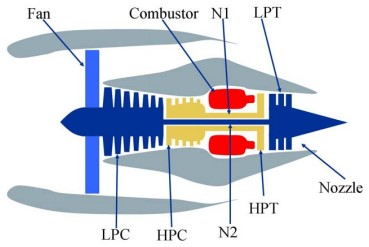
\includegraphics[width=.48\textwidth]{figures/c-mapss-engine-diagram.jpg}
    \caption{Schéma simplifié d'un turboréacteur simulé dans C-MAPSS \cite{Saxena2008}}
    \label{figure:c-mapss-engine-diagram}    
\end{wrapfigure}

Le logiciel C-MAPSS est composé de nombreux paramètres d'entrée éditables qui contrôlent la simulation. Ces entrées sont spécifiées par l'utilisateur et contrôlent de nombreux aspects de la simulation tels que le profil opérationnel, les contrôleurs en boucle fermée, les conditions environnementales, etc. \cite{Saxena2008}. 

La figure \ref{figure:c-mapss-engine-diagram} est un diagramme simplifié du turboréacteur simulé montrant ses principaux éléments, comme la section de compresseur basse pression (LPC), la section de compresseur haute pression (HPC), la soufflante et la chambre de combustion. L'ensemble de données publié par le Centre de recherche Ames de la NASA contient les données résultant de la simulation de nombreux turboréacteurs, depuis le début du fonctionnement jusqu'à la panne. L'ensemble de données a été initialement publié pour la compétition de Pronostics et gestion de la santé 2008. Le tableau \ref{table:c-mapss-sensors} montre différentes variables, la sortie de la simulation et leurs unités, qui ont été fournies pour les participants à la compétition :

\begin{table}[ht]
    \centering
    \begin{tabu}{lll}
		\tabucline[1.5pt]{-} 
        \textbf{Symbol} & \textbf{Description} & \textbf{Units}\\
        \hline
        \textbf{T2} & Total temperature at fan inlet & R \\
        \textbf{T24} & Total temperature at LPC outlet & R \\
        \textbf{T30} & Total temperature at HPC outlet & R  \\
        \textbf{T50} &Total temperature at LPT & R\\
        \textbf{P2} & Pressure at fan inlet& psia\\
        \textbf{P15}& Total pressure in bypass-duct& psia\\
        \textbf{P30}& Total pressure at HPC outlet& psia\\
        \textbf{Nf}& Physical fan speed& rpm\\
        \textbf{Nc} & Physical core speed &rpm\\
        \textbf{epr}& Engine pressure ratio (P50/P2)& --\\
        \textbf{Ps30}& Static pressure at HPC outlet& psia\\
        \textbf{phi}& Ratio of fuel flow to Ps30& pps/psi\\
        \textbf{NRf}& Corrected fan speed &rpm\\
        \textbf{NRc}& Corrected core speed& rpm\\
        \textbf{BPR}& Bypass Ratio& --\\
        \textbf{farB}& Burner fuel-air ratio &--\\
        \textbf{htBleed}& Bleed Enthalpy &-- \\
        \textbf{Nf\_dmd} &Demanded fan speed& rpm\\
        \textbf{PCNfR\_dmd}& Demanded corrected fan speed &rpm\\
        \textbf{W31} & HPT coolant bleed & lbm/s \\
        \textbf{W32} & LPT coolant bleed & lbm/ \\
		\tabucline[1.5pt]{-} 
    \end{tabu}
    \caption{Sortie de simulation C-MAPSS pour mesurer la réponse du système}
    \label{table:c-mapss-sensors}
\end{table}

La base de données C-MAPSS contient 4 ensembles : FD001, FD002, FD003 et FD004. Chaque ensemble a des conditions de travail et des modes de défaillance différents. Le tableau \ref{table:c-mapss-statistics} contient les statistiques des différents ensembles :

\begin{table}[ht]
    \centering
    \begin{tabu}{ccccc}
        
		\tabucline[1.5pt]{2-5} 
                    & units number  & max length    & average length    & min length    \\
       \hline
            FD001   & 100           & 362           & 206.31            & 128           \\
            FD002   & 260           & 378           & 206.77            & 128           \\
            FD003   & 100           & 525           & 247.2             & 145           \\
            FD004   & 249           & 543           & 245.95            & 128           \\
		\tabucline[1.5pt]{-} 
    \end{tabu}
    \caption{Statistiques sur le nombre d'unités et la longueur des cycles dans la base de données C-MAPSS.}
    \label{table:c-mapss-statistics}
\end{table}

\section{Visualisation de la dégradation des turboréacteurs}
La visualisation des résultats de la simulation peut donner une idée de la façon dont ces variables changent pendant la durée de vie du turboréacteur. La figure \ref{fig:sensors-plot} montre quatre capteurs différents de l'un des moteurs (les valeurs sont normalisées) :

\begin{figure}[h]
    \centering
    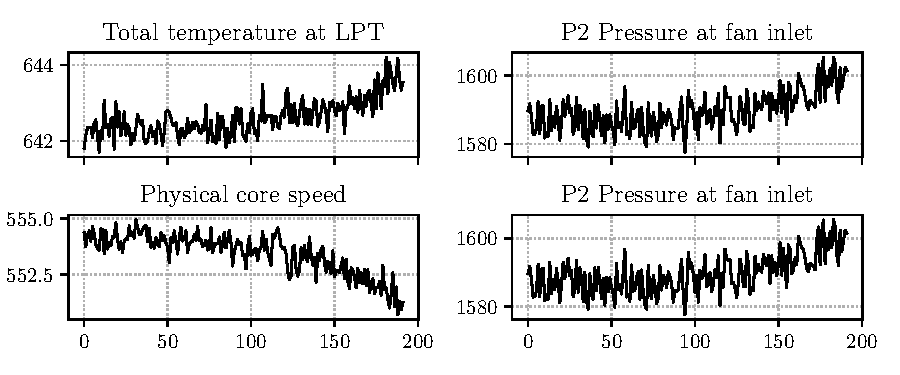
\includegraphics[width=\linewidth]{figures/sensors_plot.pdf}
    \caption{Développement de 6 capteurs de sortie d'un des turboréacteurs (normalisé)}
    \label{fig:sensors-plot}
\end{figure}
\begin{figure}[H]
    \centering
    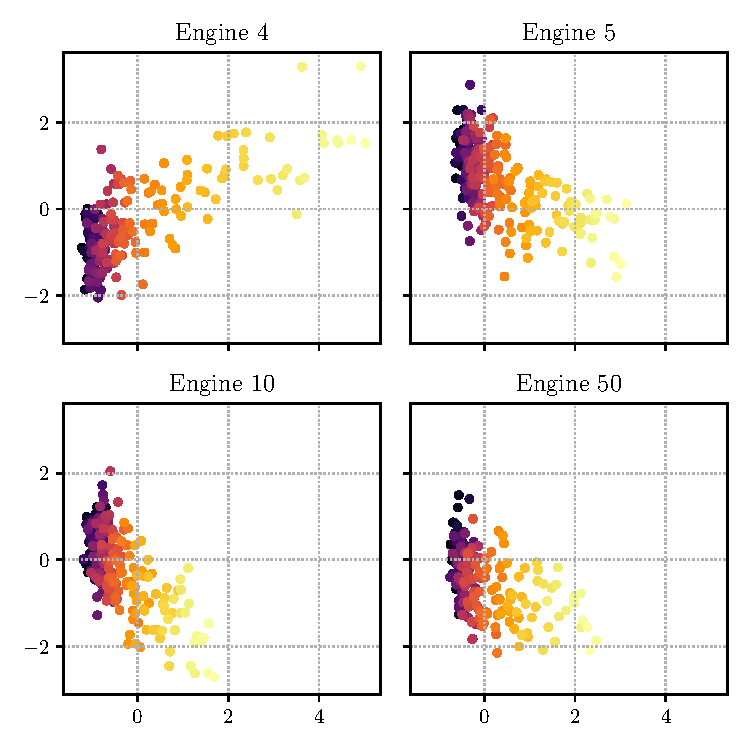
\includegraphics[width=.9\linewidth]{figures/pca-degradation.pdf}
    \caption{Dégradation de la santé de l'équipement (des couleurs plus claires indiquent l'avancement de la dégradation de la santé) de quatre turboréacteurs à partir de la base de données C-MAPSS}
    \label{fig:pca-degradation}
\end{figure}

Il est évident que la sortie des capteurs suit un tendance spécifique (croissant ou décroissant) du début de l'opération jusqu'à la panne, ce qui est très utile et peut augmenter la fiabilité du modèle prédictif.

Alternativement, toutes les valeurs des capteurs peuvent être combinées et visualisées ensemble en utilisant l'analyse en composantes principales (section \ref{section:dimensionality-reduction}) pour révéler la tendance générale des données. Si les données de surveillance de l'état de santé de l'équipement sont directement indicatives de l'état de santé de l'équipement, la visualisation des composantes principales peut montrer des modèles de dégradation visuelle apparents.

Les valeurs des capteurs de 4 turboréacteurs différents sont combinées à l'aide de l'ACP et les deux premiers composants principaux sont représentés sur la figure \ref{fig:pca-degradation}. 

Il existe un schéma absolument apparent de dégradation de l'état de santé dans les différentes unités, de la gauche (où les couleurs plus foncées indiquent un état de fonctionnement normal) à la droite (où les couleurs plus claires indiquent le développement de défauts).

\section{classification de l'état de santé des turboréacteurs}
Avant de procéder à une tâche compliquée telle que l'estimation \acrshort{rul}, une tâche plus simple comme la classification sanitaire des turboréacteurs peut montrer la complexité du problème. Cette section décrit l'utilisation des réseaux de neurones pour classer les états des moteurs comme étant sains ou défectueux. Les 25 premiers et derniers cycles de chaque unité sont considérés comme sains et défectueux respectivement.

Un réseau de neurones qui utilise les 24 entrées (tous les paramètres opérationnels et les capteurs) avec deux couches cachées est utilisé pour effectuer cette classification. Le tableau \ref{table:c-mapss-classifier-architecture} résume l'architecture du réseau :

\begin{table}[ht]
    \centering
    \begin{tabu}{lll}
		\tabucline[1.5pt]{-}
		\textbf{Couche (type)}   & \textbf{Forme de la sortie} &   \textbf{Param \#} \\
		\tabucline[1pt]{-}
		Dense1 (Dense) 			&   (None, 8)   &   200\\
		Dense2 (Dense) 	        &   (None, 4)   &   36       \\
		Dense3 (Dense)			&   (None, 1)   &   5   \\
		\tabucline[1pt]{-}
		Total params: 241       &                   &           \\
		Trainable params: 241   &                   &           \\
		Non-trainable params: 0     &                   &           \\
	\tabucline[1.5pt]{-}
    \end{tabu}
    \caption{Architecture du classificateur de l'état des unités}
    \label{table:c-mapss-classifier-architecture}
\end{table}

Le modèle est entraîné pour 200 époques avec batch size de 32 échantillons, le classificateur atteint une exactitude de \textbf{93,46\%} sur les données de test. La figure \ref{fig:cmapss-classifier-training} montre le processus d'entraînement du réseau. Dans le diagramme du haut, l'axe des y correspond aux pertes d'entraînement et de validation (crossentropie binaire). L'axe des y dans le diagramme du bas correspond aux précisions d'entraînement et de validation du réseau, l'axe des x partagé entre les deux diagrammes indique les époques de formation. Bien que l'exactitude de validation varie beaucoup, l'exactitude d'entraînement continue de s'améliorer à chaque époque.

\begin{figure}[H]
    \centering
    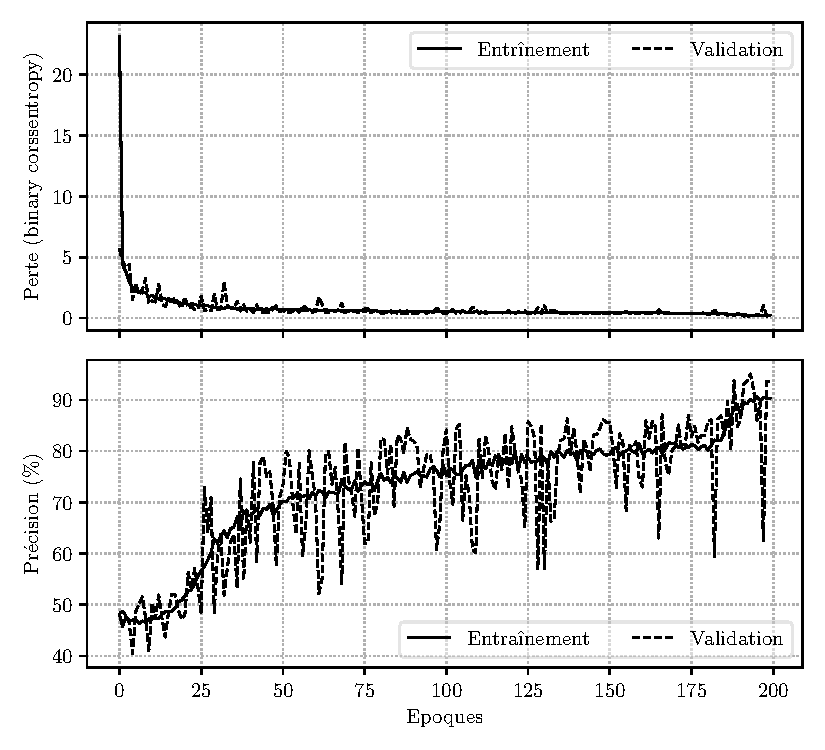
\includegraphics{figures/cmapss_classification_training_fr.pdf}
    \caption{Processus d'entraînement du classificateur de l'état des unités}
    \label{fig:cmapss-classifier-training}
\end{figure}

La figure \ref{fig:cmapss-classifier-roc} montre la courbe \acrlong{roc} (\acrshort{roc}) du classificateur avec un haut \acrlong{auc} (\acrshort{auc}). D'autres mesures de classification sont présentées dans le tableau \ref{table:cmapss-classifier-metrics}.

\begin{figure}[H]
    \centering
    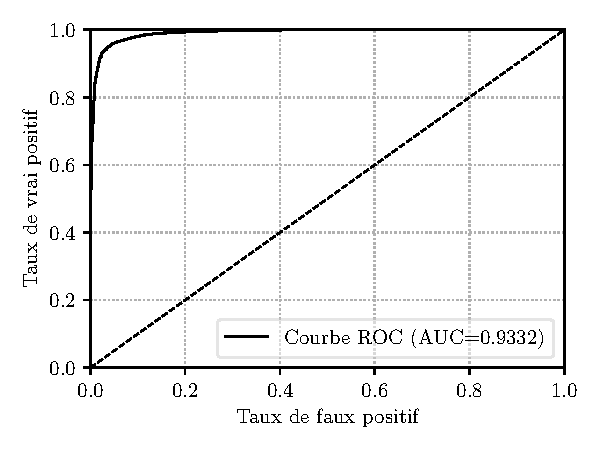
\includegraphics{figures/cmapss_classification_roc_fr.pdf}
    \caption{Courbe \acrshort{roc} du classificateur sur les données de test}
    \label{fig:cmapss-classifier-roc}
\end{figure}

\begin{table}[H]
    \centering
    \begin{tabu}{cccccc}
        
    \tabucline[1.5pt]{-}
    \textbf{Métrique} &  \textbf{Exactitude} &  \textbf{Précision} &  \textbf{Rappel} &  \textbf{F-1} &  \textbf{ROC AUC}  \\
    \hline
    \textbf{Valeur} & 93.43\% & 0.90 & 0.98 & 0.94 & 0.9332 \\
	\tabucline[1.5pt]{-}
    \end{tabu}
    \caption{Métriques du classificateur sur les données de test}
    \label{table:cmapss-classifier-metrics}
\end{table}

\section{Prédiction de \acrshort{rul}}
\subsection{Modèlisation de \acrshort{rul}}

Afin d'entraîner un réseau de neurones pour l'estimation de  \acrlong{rul} (\acrshort{rul}) d'une nouvelle donnée non vue provenant de base de données C-MAPSS, un \acrshort{rul} approprié correspondant aux données d'entraînement doit être construit.

L'expression \acrshort{rul} a été définie dans la section \ref{section:rul}, à partir de cette définition, plusieurs approches pour construire un \acrshort{rul} approprié peuvent être développées pour les unités dans les données d'entraînement (où le nombre total de cycles avant la défaillance est connu). L'approche la plus simple consiste à utiliser un \acrshort{rul} toujours décroissant, ce qui implique que l'état de l'équipement est toujours décroissant et va vers la défaillance.

Le problème de cette approche est que le processus de dégradation n'est pas linéaire et que dans la vie réelle, les machines ne commencent pas à se dégrader dès qu'elles commencent à fonctionner. Une deuxième approche consiste à utiliser une fonction par morceaux où l'état de l'équipement est d'abord constant puis, à un point spécifique, il commence à se dégrader de manière linéaire.

Cette approche est bien meilleure que la première, mais elle n'est pas très représentative du comportement réel du processus de dégradation. Dans le contexte de ce mémoire, \acrshort{rul} est abordé comme une fonction polynomiale non linéaire où la dégradation est lente au début puis s'accélère vers la fin de la vie. La figure \ref{fig:rul-models} montre les différents choix de modélisation de \acrshort{rul} :

\begin{figure}[H]
    \centering
    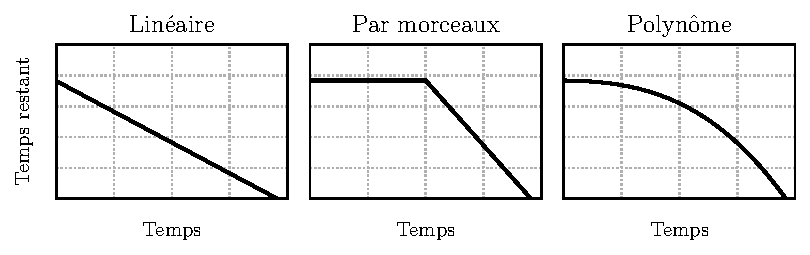
\includegraphics{figures/rul_models_fr.pdf}
    \caption{Différents modèles de \acrshort{rul}}
    \label{fig:rul-models}
\end{figure}

Il convient de noter qu'aucune de ces approches ne peut être considérée comme représentative du processus de dégradation réel, mais le choix de la représentation la plus intuitive de \acrshort{rul} peut aider l'algorithme d'apprentissage à connaître les tendances de dégradation implicites dans les données.

\subsection{Prédiction de \acrshort{rul} par un réseau de neurones}

La dernière section portait sur la classification de l'état de santé des unités comme étant sain ou défectueux. Cette section présente plutôt un réseau de neurones pour l'estimation de la \acrshort{rul}. Dans cette section, une architecture de réseau de neurones avec 3 couches cachées est utilisée. Comme il s'agit d'un problème de régression, l'erreur quadratique moyenne est utilisée comme fonction de perte, l'erreur absolue moyenne est utilisée comme mesure pour le modèle. Le tableau \ref{table:cmapss-regression-architecture} présente les détails de l'architecture :

\begin{table}[h]
    \centering
    \begin{tabu}{lll}
		\tabucline[1.5pt]{-}
		\textbf{Couche (type)}   & \textbf{Forme de la sortie} &   \textbf{Param \#} \\
		\tabucline[1pt]{-}
		Dense1 (Dense) 			&   (None, 32)  &       800     \\
		Dense2 (Dense)          &   (None, 16)  &       528     \\
		Dense3 (Dense)          &   (None, 8)   &       136     \\
		Dense4 (Dense)          &   (None, 1)   &       9       \\

		\tabucline[1pt]{-}
		Total params: 1,473       &                   &           \\
		Trainable params: 1,473   &                   &           \\
		Non-trainable params: 0   &                   &           \\
	\tabucline[1.5pt]{-}
    \end{tabu}
    \caption{Architecture d'un réseau de neurones pour la prédiction de \acrshort{rul}}
    \label{table:cmapss-regression-architecture}
\end{table}

Le réseau a été entraîné pour 300 époques, avec batch size de 128 échantillons. La figure \ref{fig:cmapss-regression-training} montre le processus de'entraînement du réseau. Les figures montrent l'évolution des pertes d'entraînement et de validation (erreur quadratique moyenne) et des métriques (erreur absolue moyenne) respectivement en fonction des époques.

\begin{figure}[H]
    \centering
    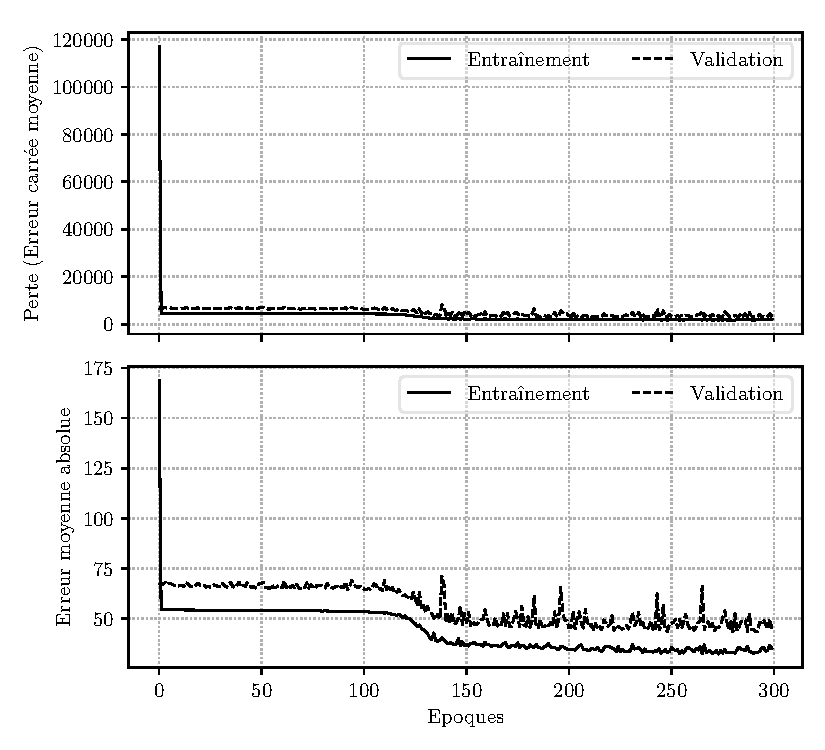
\includegraphics{figures/cmapss_regression_training_fr.pdf}
    \caption{Processus d'entraînement du réseau utilitsé pour prédire \acrshort{rul}}
    \label{fig:cmapss-regression-training}
\end{figure}

Après l'entraînement, le modèle est évalué sur deux unités de la série de tests. La figure \ref{fig:cmapss-regression-prediction} montre le \acrshort{rul} réel (ligne discontinue), la prédiction du modèle à chaque cycle et un ajustement polyomial de 3ème degré des prédictions du modèle.

\begin{figure}[H]
    \centering
    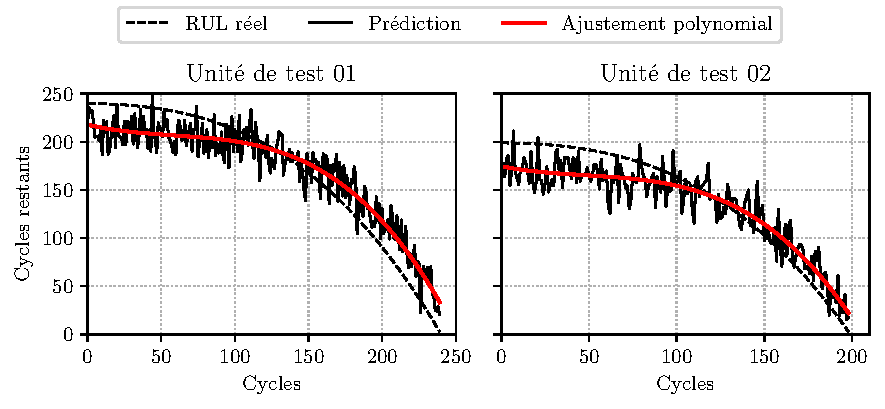
\includegraphics{figures/cmapss_regression_predictions_fr.pdf}
    \caption{Résultats de prédiction de \acrshort{rul} par un réseau de neurones}
    \label{fig:cmapss-regression-prediction}
\end{figure}

Bien que les prévisions du modèle soient proches de la réalité, mais elles sont bruyantes et il y a beaucoup de fluctuation. Le bruit peut être réduit en lissant la sortie, par exemple en utilisant une moyenne mobile ou en adaptant les points à un polynôme. Mais la raison du bruit en premier lieu est que l'architecture entièrement connectée ne prend pas en considération les prédictions précédentes (c'est-à-dire l'architecture acyclique). Étant donné qu'à chaque instant, la \acrshort{rul} dépend de la \acrshort{rul} de la précédente, le fait de prendre en considération les étapes précédentes tout en faisant de nouvelles prédictions peut effectivement réduire le bruit et aussi améliorer la précision des prédictions. Pour y parvenir, il convient d'utiliser une architecture neurale cyclique comme les réseaux de neurones récurrents.

\subsection{Amélioration de la prédiction \acrshort{rul} en utilisant les réseaux LSTM}

Les réseaux de neurones entièrement connectés constituent un outil puissant pour la modélisation d'un large éventail de problèmes, mais l'utilisation de cette architecture pour la prédiction de séries chronologiques, comme la prédiction \acrshort{rul}, peut donner un résultat très bruyant car le réseau est acyclique et chaque instant dans le temps est évalué séparément et ne tient pas compte des prédictions précédentes. \acrlong{lstm} (Section \ref{section:lstm}) est un outil puissant pour modéliser de tels problèmes et pour faire des prédictions plus fiables et moins bruyantes. Dans cette section, l'architecture de réseau de neurones entièrement connectée de la section précédente est remplacée par un réseau \acrshort{lstm} pour prédire \acrshort{rul} des turboréacteurs de la base de données C-MAPSS.

L'architecture utilisée ici est décrite dans le tableau \ref{table:cmapss-lstm-architecture}:

\begin{table}[h]
    \centering
    \begin{tabu}{lll}
		\tabucline[1.5pt]{-}
		\textbf{Couche (type)}   & \textbf{Forme de la sortie} &   \textbf{Param \#} \\
		\tabucline[1pt]{-}
		LSTM1 (LSTM) 			&   (None, 100, 100)    &       50000   \\
		LSTM2 (LSTM)           &   (None, 100, 100)    &       80400   \\
		LSTM3 (LSTM)           &   (None, 75)          &       52800   \\
        Dense1 (Dense)         &   (None, 120)         &       9120    \\
        Dense2 (Dense)         &   (None, 110)         &       13310   \\
        Dense3 (Dense)         &   (None, 100)         &       11100   \\
		\tabucline[1pt]{-}
		Total params: 216,730       &                   &               \\
		Trainable params: 216,730   &                   &               \\
		Non-trainable params: 0     &                   &               \\
	\tabucline[1.5pt]{-}
    \end{tabu}
    \caption{Architecture de réseau \acrshort{lstm} pour la prédiction de \acrshort{rul}}
    \label{table:cmapss-lstm-architecture}
\end{table}

Il est évident que l'architecture \acrshort{lstm} a beaucoup plus de paramètres (216,730 paramètres) que l'architecture entièrement connectée (1,473). Cela est dû à la conception plus complexe des cellules \acrshort{lstm} et à leur possession de différentes portes. Il en résulte un temps d'entraînement beaucoup plus long.

Les couches \acrshort{lstm} prennent un tenseur tridimensionnel de la forme \textit{(samples, sequence length, features)} comme entrée. La longueur de la séquence a été fixée à 100 dans cette architecture, c'est pourquoi chaque échantillon d'entraînement doit avoir une forme de \textit{(sequence length, features)}. Toutes les unités ont le même nombre de caractéristiques mais des longueurs différentes, puisque chaque échantillon doit avoir une longueur de séquence de 100, les échantillons avec des cycles inférieurs à 100 sont complétés par -10 où les couches \acrshort{lstm} sont définies pour ignorer tout les instants de temps avec cette valeur.

Le réseau a été entraîné pour 50 époques avec batch size de 16 échantillons et un fractionnement de validation de 0,2 en utilisant l'algorithme d'optimization Adam. Le processus d'entraînement est visualisé sur la figure \ref{fig:cmapss-lstm-training} :

\begin{figure}[H]
    \centering
    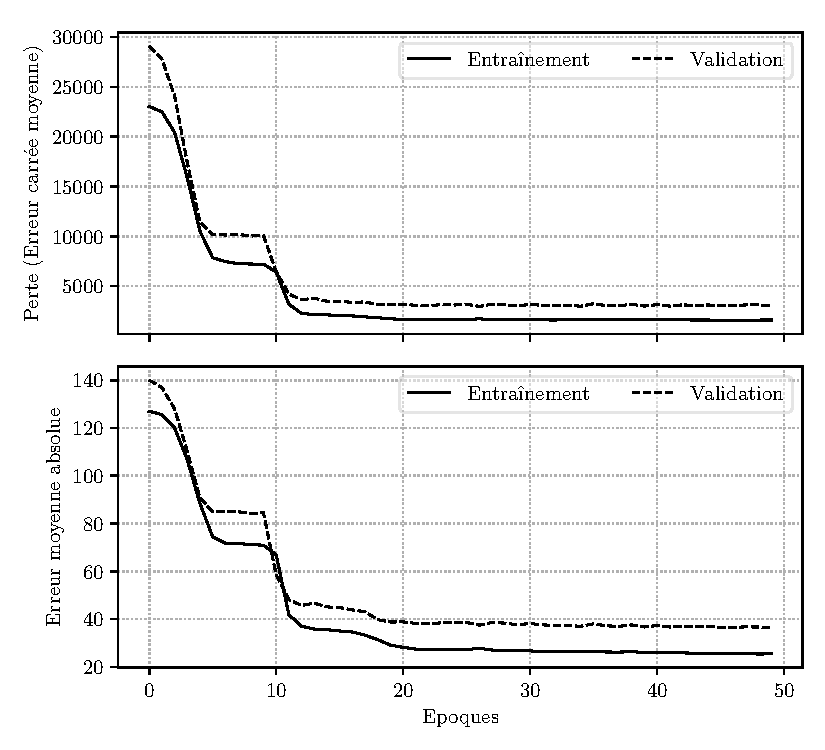
\includegraphics{figures/cmapss_lstm_training_fr.pdf}
    \caption{Processus d'entraînement du réseau \acrshort{lstm}}
    \label{fig:cmapss-lstm-training}
\end{figure}

Le tableau \ref{table:cmapss-lstm-results} montre la perte et la métrique (c'est-à-dire l'erreur absolue moyenne) sur les donnée d'entraînement, validation et de test :

\begin{table}[H]
	\centering
	\begin{tabu}{lcc}
		\tabucline[1.5pt]{2-3} 
						&	\textbf{Perte}	&	\textbf{Erreur absolue moyenne}	\\
	   \tabucline[1pt]{-}
		Ensemble d'entraînement 		&	1600.60			    &	25.43				\\
		Ensemble de validation 	&	3039.68 			&	36.37					\\
		Ensemble de test		&	1379.67 			&	23.27					\\
   \tabucline[1.5pt]{-}
   \end{tabu}
   \caption{Résultats d'entraînement du réseau\acrshort{lstm}}
   \label{table:cmapss-lstm-results}
\end{table}

Quatre unités différentes ont été réservées comme unités de test. Après l'entraînement, le réseau est utilisé pour prédire \acrshort{rul} sur les unités de test. La figure \ref{fig:cmapss-lstm-prediction} montre les résultats de la prédiction et la \acrshort{rul} réelle de deux unités différentes :

\begin{figure}[h]
    \centering
    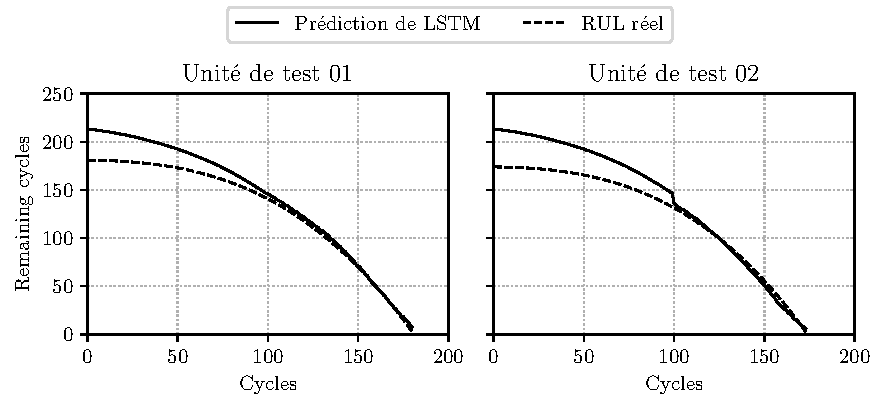
\includegraphics{figures/cmapss_lstm_regression_predictions_fr.pdf}
    \caption{Résultats de prédiction du réseau \acrshort{lstm}}
    \label{fig:cmapss-lstm-prediction}
\end{figure}

Il est évident que les prédictions du réseau \acrshort{lstm} sont bien meilleures et presque exemptes de bruit par rapport à celles faites par le réseau entièrement connecté, comme le montre la figure \ref{fig:cmapss-regression-prediction}. La prédiction \acrshort{rul} est presque identique à la prédiction réelle \acrshort{rul} vers la fin de vie du turboréacteur.

\section{Application aux équipements des chantiers pétroliers}%
\label{sec:application_to_oilfield_equipment_1}
Ce chapitre a présenté une approche de maintenance prédictive pour l'estimation des \acrshort{rul} basée sur les données de surveillance de l'état fournies par différents capteurs qui peuvent mesurer différentes variables physiques qui sont liées à l'état de santé de l'équipement. Les données utilisées dans les sections précédentes consistaient en une base de données de turboréacteurs C-MAPSS, mais la même approche peut être étendue à d'autres applications comme les plates-formes pétrolières.

Les chantiers pétroliers modernes contiennent un grand nombre de capteurs répartis sur presque tous les équipements critiques. Ces capteurs mesurent différentes variables physiques telles que la température, le débit, la pression…. Mais la majorité des données fournies par ces capteurs n'est pas correctement exploitée dans un cadre approprié de pronostics et de maintenance prédictive. Il existe d'énormes quantités de données historiques dans les chantiers pétroliers qui, si elles sont exploitées, peuvent améliorer considérablement les programmes de maintenance dans des applications aussi critiques où la réduction des temps d'arrêt est très importante et où l'indisponibilité des équipements peut avoir causé des pertes de production importantes.

\begin{figure}[p!]
	\centering
	\includegraphics[width=0.9\linewidth]{figures/honeywell-oilrig-sensors.png}
	\caption{Emplacement des capteurs dans un chantier pétrolier \cite{honeywellrig}}%
	\label{fig:honeywell-oilrig-sensors}
\end{figure}

La figure \ref{fig:honeywell-oilrig-sensors} montre différents endroits où les capteurs sont installés sur la plupart des chantiers pétroliers modernes. Le tableau \ref{table:honeywell-oilrig-sensors} énumère les types de différents capteurs qui peuvent être utilisés pour les pronostics, les unités auxquelles ils sont attachés et les variables physiques qu'ils peuvent mesurer. Un réseau de neurones peut être entraîné sur les données historiques de la plate-forme et être utilisé pour surveiller les différents équipements, leur interaction, détecter les anomalies et les signaler à temps afin de mener les actions de maintenance appropriées.

\begin{table}[p!]
	\centering
	\begin{adjustbox}{angle=90}
	\begin{tabu}{clp{30mm}p{120mm}}
		\tabucline[1.5pt]{-} 
		\textbf{Capteur} & \textbf{Equipment} & \textbf{Type de capteur}  & \textbf{Value mesurée}\\
        \hline
A&	Crown Block &	Load cell	&	Weight on drill line via cable tension\\
B& Power Generation Unit	&	Pressure&	Oil, water, and hydraulic fluid pressure\\
D&Accumulator Unit	&	Pressure&	Inlet/outlet pressure with high accuracy\\
F&Rig Hydraulic Lift	&	Pressure&	Hydraulic pressure, weight, force/strain, or movement, monitor raising or lowering deck for directional drilling\\
H&Drawworks	&	Load cells	&	Torque, load/weight/position while guiding pipe into position\\
M&Water/Storage Tank	&	Pressure& Tank liquid levels\\
N&Top Drive	&	Torque/Pressure&	Monitor torque/twisting movement to ensure right amount of force is applied. Weight on drill bit. Hydraulic pressure and feed information into control system.\\
O&Trabeling Block	&	Load cells	&	Weight on the drill line via cable tension\\
R&Deadline anchor	&	Load cells	&	Tension on deadline/drilling line cable\\
U&Mud Return Line	&	Pressure&	Drilling mud pressure to monitor and control mud flow\\
Y&Mud Pump	&	Pressure&	Pressure and flow of mud media\\
AB&BlowOut Preventor &	Pressure&	Monitor RAM position via hydraulic volumetric or pressure behind the piston\\
AD&Drill Bit	&	Pressure&	Pressure or differential pressure at high temperature and pressure ranges\\
AE	&	Fluid manifold	&	Pressure	&	Drilling fluid pressure\\
AF&Mud Tank/Reservoir	&	Pressure&	Tank liquid levels\\
		\tabucline[1.5pt]{-} 
    \end{tabu}
\end{adjustbox}
    \caption{Liste des capteurs dans un chantier pétrolier \cite{honeywellrig}}
    \label{table:honeywell-oilrig-sensors}

\end{table}

\section{Conclusion}
Les réseaux de neurones entièrement connectés sont un outil puissant pour quantifier l'état de santé de systèmes complexes à l'aide de données de surveillance des conditions. L'ensemble de données C-MAPSS est un exemple de système comportant de nombreuses parties en interaction qui fournissent une variété de données de surveillance de l'état de santé (par exemple, la température, la pression, le régime, ...) où la dégradation n'est pas directement liée à une composante mais est indiquée par la somme des tendances de toutes les données de surveillance. Les réseaux de neurones sont capables de saisir de telles tendances et de prédire \acrshort{rul} du système avant une défaillance. Les réseaux entièrement connectés ont d'abord été utilisés pour cette tâche, mais une architecture cyclique comme \acrshort{lstm} peut produire de meilleurs résultats avec une précision accrue et beaucoup moins de bruit. Une approche pour integrer les réseaux de neurones dans le cadre de maintenance préventive et pronostic dans les chantiers pétroliers en exploitant les différents capteurs et les données historiques disponibles pour créer un programme de maintenance plus fiable et moderne.
